

\documentclass{article}

\usepackage{url,graphicx,tabularx,array,geometry, hyperref}
\usepackage{listings}
\usepackage{fullpage}
\usepackage{fancyvrb}
\usepackage{framed}
\usepackage{lastpage}
\usepackage{fancyhdr}
\usepackage{color}
\usepackage{tabu}
\usepackage[doi=true,style=ieee,backend=bibtex]{biblatex}
\bibliography{sauce}
\def\tablename{Table}

\definecolor{codegreen}{rgb}{0,0.6,0}
\definecolor{codegray}{rgb}{0.5,0.5,0.5}
\definecolor{codepurple}{rgb}{0.58,0,0.82}
\definecolor{backcolour}{rgb}{0.95,0.95,0.92}

\lstdefinestyle{mystyle}{
    backgroundcolor=\color{backcolour},   
    commentstyle=\color{codegreen},
    keywordstyle=\color{magenta},
    numberstyle=\tiny\color{codegray},
    stringstyle=\color{codepurple},
    basicstyle=\footnotesize,
    breakatwhitespace=false,         
    breaklines=true,                 
    captionpos=b,                    
    keepspaces=true,                 
    numbers=left,                    
    numbersep=5pt,                  
    showspaces=false,                
    showstringspaces=false,
    showtabs=false,                  
    tabsize=2
}
% http://gnuplot.sourceforge.net/docs_4.2/node237.html
\lstset{style=mystyle}

\renewcommand{\headrulewidth}{0pt}
\setcounter{secnumdepth}{0}

\setlength{\parskip}{1ex} %--skip lines between paragraphs
\setlength{\parindent}{0pt} %--don't indent paragraphs
\setlength{\headheight}{15.2pt}

\pagestyle{fancy}

\renewcommand{\headrulewidth}{0pt}
\lhead{  }
\lfoot{Lab 1: TCP Congestion Control}
\rfoot{page \thepage\ of \pageref{LastPage}}

\renewcommand{\familydefault}{\sfdefault}
\begin{document}

\begin{titlepage}
\begin{center}
\textsc{\huge \bfseries Advanced Networking 2018}\\[1.5cm]
\textsc{\large Lab \#1: TCP Congestion Control}\\[1.5cm]
\textsc{\huge Report}\\[1.5cm]
\textsc{\huge \bfseries GROUP: 11}\\[1.5cm]
\textsc{\large{\textbf{Authors:}\\ Sjors Haanen, Sjors.Haanen@os3.nl\\ Péter Prjevara, Peter.Prjevara@os3.nl}}

\textsc{\large University of Amsterdam}
\end{center}
\end{titlepage}

\begin{lstlisting}[caption=<EXAMPLE>]
config.vm.synced_folder "src/", "/home/vagrant/ns-allinone-3.27/ns-3.27/task1"
\end{lstlisting}

\subsection{Preparation}

To share files from host to guest, we used Vagrants Synched Folders functionality by putting the following line in the VagrantFile:

\begin{lstlisting}[caption=Vagrant Synched Folders config]

\end{lstlisting}

\subsection{Q1.1 Plot a graph showing CWND versus time from 0.0s to
100.0s.}

\begin{figure}[h]
    \centering
    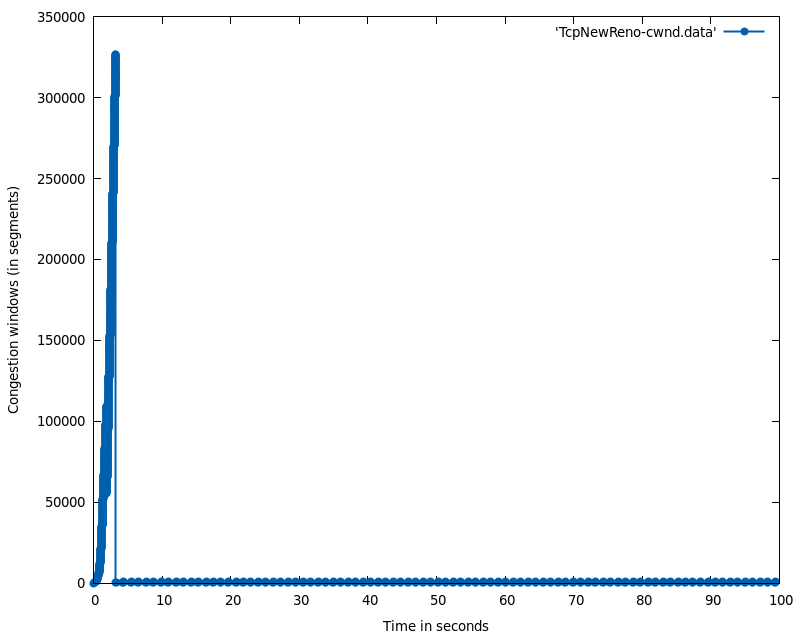
\includegraphics[scale=0.5]{images/lab1-group11-task1-question1.png}
    \caption{CWND versus time}
    \label{fig:q1-1}
\end{figure}

\newpage

\subsection{Q1.2 Plot a graph showing SSTH versus time from 0.0s to
100.0s.}

\begin{figure}[h]
    \centering
    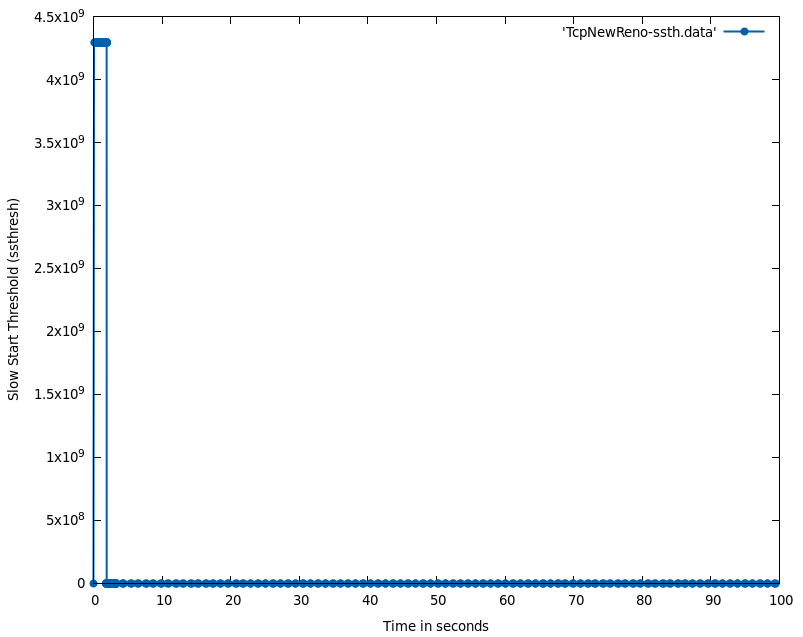
\includegraphics[scale=0.5]{images/lab1-group11-task1-question2.png}
    \caption{SSTH versus time}
    \label{fig:q1-2}
\end{figure}

\newpage

\subsection{Q1.3 Find the points where the slow-start,
congestion-avoidance, fast retransmit/fast recovery states begin.}

\begin{table}
\begin{tabular}{|c|p{25mm}|p{20mm}|c|c|}
\hline Time (s)    & Current CWND (bytes)    & New CWND (bytes)    & New State    & Event \\
\hline 0.0       &         0.0     &     340     &       Slow Start      &  Transmission Start\\ 
\hline 1.932     &      109480     &    55590    &       Fast Recovery   &  DupAckCounter == 3\\
\hline up to 3.269 &    x          &  x - 3xMSS  &       Fast Recovery   &  NewAckReceived\\
\hline 3.269     &      326570     &     340     &       Slow Start      &  Timeout\\ 
\hline 3.308     &      680        &     680     &       Fast Recovery   &  DupAckCounter == 3\\   
\hline 4.309     &      680        &     340     &       Slow Start      &  Timeout\\ 
\hline 4.309     &      680        &     680     &       Congestion Avoidance   &  SSTH == CWND\\ 
\hline 4.395     &      850        &     340     &       Slow Start      &  Timeout\\
\hline 4.395 until recovery     &      repeat prev two steps       &  ...  & ...  &  ... \\
\hline
\end{tabular} 
\end{table}

The following charts depict the above events happening well in detail:

\begin{figure}[h]
    \centering
    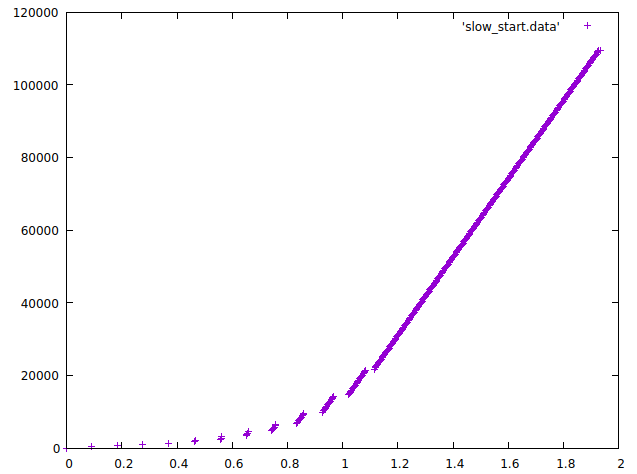
\includegraphics[scale=0.4]{images/lab1-group11-task1-question3-1.png}
    \caption{First Slow Start Phase}
    \label{fig:slow_start}
\end{figure}

The first slow start phase ends when the 3rd DupAck is received. This results in the SSTH to reduce to current CWND/2, to 54570. The new CWND will be this value + 3*MSS (54570 + 1020 = 55590).\\

Figure 5 depicts the Fast Recovery state happening afterwards. The sender enters to into Fast Recovery State, and stays in Fast Recovery until 3.269. It can be seen however that each time a NewAck is received from the receiver, CWND deflation occurs, because the NewAck is only covering part of the current FlightSize.

\begin{figure}[h]
    \centering
    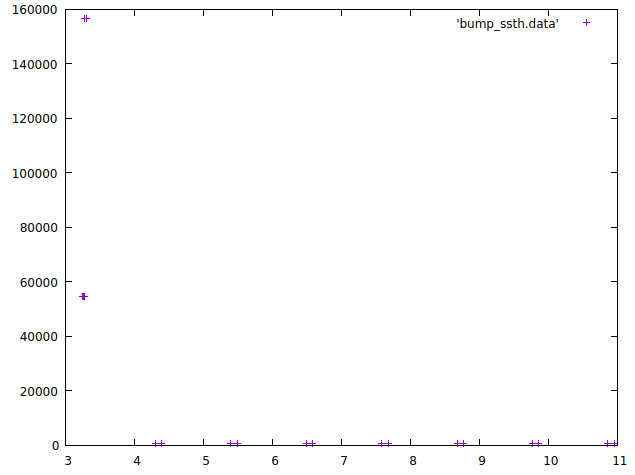
\includegraphics[scale=0.4]{images/lab1-group11-task1-question3-2.png}
    \caption{SSTH Bump - Transition from Slow Start to Fast Recovery then to Slow Start last}
    \label{fig:ssth_bump}
\end{figure}

\begin{figure}[h!]
    \centering
    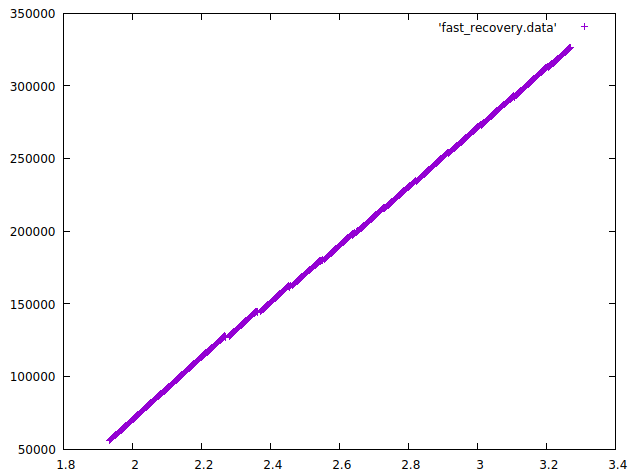
\includegraphics[scale=0.4]{images/lab1-group11-task1-question3-3.png}
    \caption{Fast Recovery Phase with CWND Deflation}
    \label{fig:cwnd_deflation}
\end{figure}

At the end of this chart a timeout occurs, and several timeouts arrive afterwards which is the cause of the flat line on Figure 1. Before the transmission would settle in the Slow Start process until the end, it jumps to Fast Recovery ONCE until the next timeout comes through, due to receiving 3 DupAcks (and many more) again. The following Figure 5 depicts the SSTH value at the time of this happening, proving the event taking place. On Figure 4 the first data point represents the SSTH figure of 54570, that was taken at the time when the transmission entered the Fast Recovery state for the first time. After that, due to the states jumping in between Slow Start and Fast Recovery quickly, it increases to CWND/2 (156400 at the ti
me), to then reduce to 2*MSS (680) when the timeouts start to occur. The line after the 4th sec is not fully flat on Figure 4 SSTH Bump figure: 850 - 340 - 680 - 850 - 340 - 680 - 850 ... pattern keeps happening. This proves the bounce between Congestion Avoidance and Slow Start. 
\\
These observations are underpinned through the correlation of RFC 6582, RFC 2581, the inflight.data, the cwnd.data, the ssth.data and the pcap file 1-1.
\newpage
\subsection{Q1.4 Plot a graph showing CWND versus time from 0.0s to
100.0s.}

\begin{figure}[h]
    \centering
    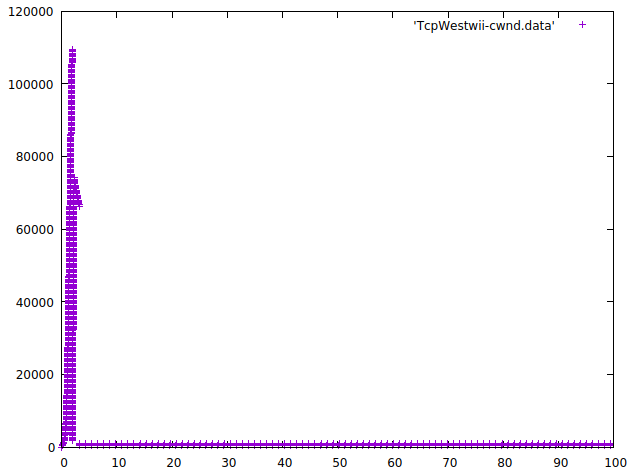
\includegraphics[scale=0.4]{images/lab1-group11-task1-question4.png}
    \caption{Westwood CWND 0-100s}
    \label{fig:cwnd_deflation}
\end{figure}

\subsection{Q1.5 Plot a graph showing SSTH versus time from 0.0s to
100.0s.}

\begin{figure}[h]
    \centering
    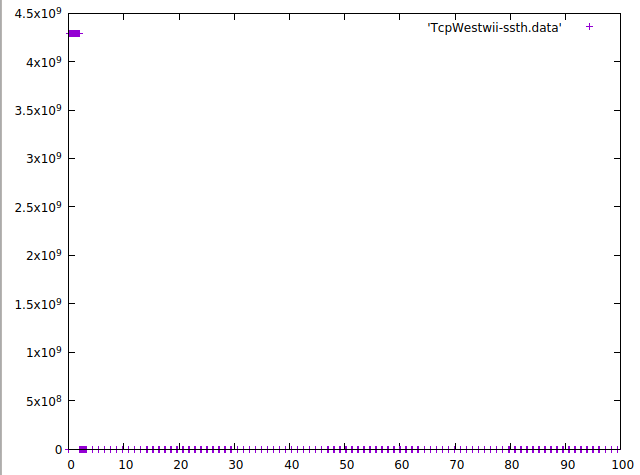
\includegraphics[scale=0.4]{images/lab1-group11-task1-question5.png}
    \caption{Westwood SSTH 0-100s}
    \label{fig:cwnd_deflation}
\end{figure}

\newpage
\subsection{Q1.6 Find the points where the slow-start,
congestion-avoidance, fast retransmit/fast recovery states begin.}

\begin{table}[h]
\begin{tabular}{|c|p{25mm}|p{20mm}|c|c|}
\hline Time (s)    & Current CWND (bytes)    & New CWND (bytes)    & New State    & Event \\
\hline 0.0       &         0.0     &     340     &       Slow Start      &  Transmission Start\\ 
\hline 1.932     &      109480     &    1700   &       Faster Recovery   &  DupAckCounter == 3\\
\hline 3.269     &      326570     &     340     &       Slow Start      &  Timeout\\ 
\hline 3.308     &      680        &     680     &       Congestion Avoidance   &  \\   
\hline
\end{tabular} 
\end{table}

The following chart nicely represents the points that matter in the process:

\begin{figure}[h]
    \centering
    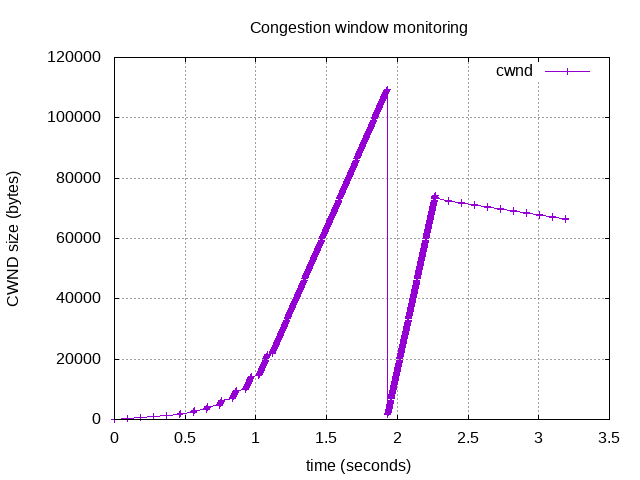
\includegraphics[scale=0.6]{images/lab1-group11-task1-question6.png}
    \caption{CWND Westwood Full}
    \label{fig:cwnd_deflation}
\end{figure}



\subsection{Q1.7 Discuss and motivate the differences you observe
between the NewReno and this algorithm.}

TCP Westwood is a server-side modification of TCP New Reno. While TCP Reno is sensitive to random loss (it cannot discriminate between them) and overreacts on it, TCP Westwood does not. TCP Westwood continuously measures the bandwidth (at the sender-side) via monitoring the rate of returning ACKs. This is used to compute congestion window and slow start threshold after a congestion happened. This way TCP Westwood attempts to select a SSTH and a CWND which are consistent with the effective bandwidth used at the time congestion is experienced. \parencite{casetti2002tcp}

More precisely, when packet loss occurred, the TCP Westwood sender sets the CWND as following:

$ CWND = RE \times RTT $

where $ RE $ is the estimate bandwidth and $ RTT $ is the Round Trip Time. This is what happends at 1.932 in our simulation.

The major difference is that the NewReno Algorithm does the deflation of CWND which does not happen in Westwood. Westwood on the other hand tries to guess the initial CWND instead of starting from 1 MSS.

\newpage

\subsection{Q2.1 Plot a graph showing the CWND and ssthresh versus time
with all the data you get. These two metrics are in one graph.}

\begin{figure}[h]
    \centering
    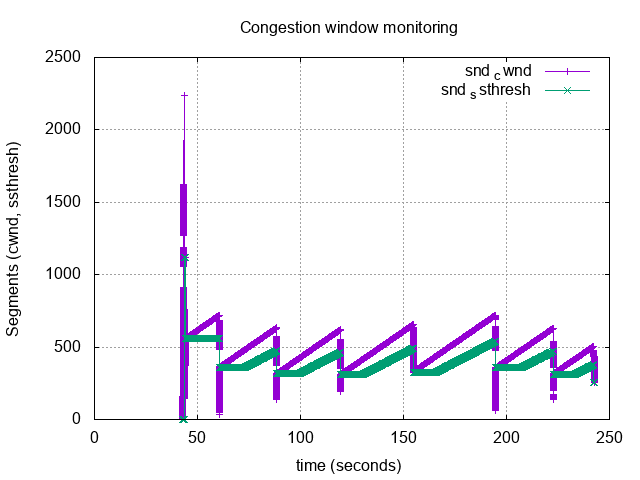
\includegraphics[scale=0.5]{images/lab1-group11-task2-question1.png}
    \caption{TCP Reno with 50ms latency and 0\% packet loss}
    \label{fig:lab1-group11-task2-question1}
\end{figure}

\begin{figure}[h!]
    \centering
    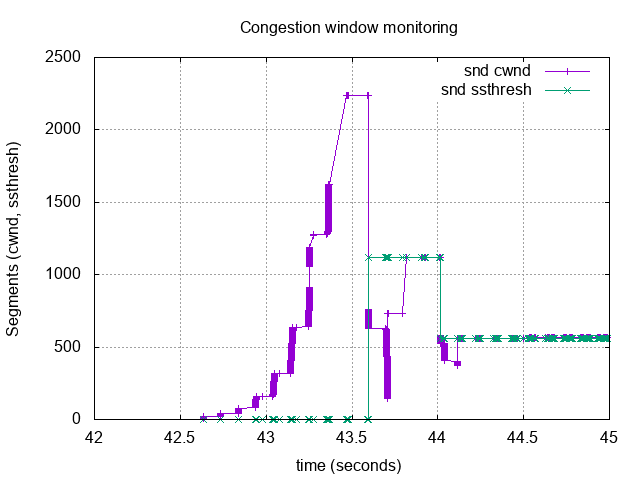
\includegraphics[scale=0.5]{images/lab1-group11-task2-question1-zoom.png}
    \caption{TCP Reno with 50ms latency and 0\% packet loss}
    \label{fig:lab1-group11-task2-question1-zoom}
\end{figure}

\subsection{Q2.2 Briefly discuss the changing process.}

As plotted in figure \ref{fig:lab1-group11-task2-question1} and \ref{fig:lab1-group11-task2-question1-zoom}, the slow start phase ends at around 2 sec of the simulation, when the SSTH becomes half the current congestion window. At that time, the DupAckCounter becomes 3 so the process goes in to Fast Recovery then Congestion Avoidance Phase. The repeating intervals are patterns of congestion avoidance and fast recovery: when 3 dup acks received the process bounces between fast recovery and congestion avoidance. This is underpinned by the fact that the CWND never returns to MSS (the original value 10).

\newpage

\subsection{Q2.3 Plot a graph showing CWND versus time with all the data
you get.}

\begin{figure}[h]
    \centering
    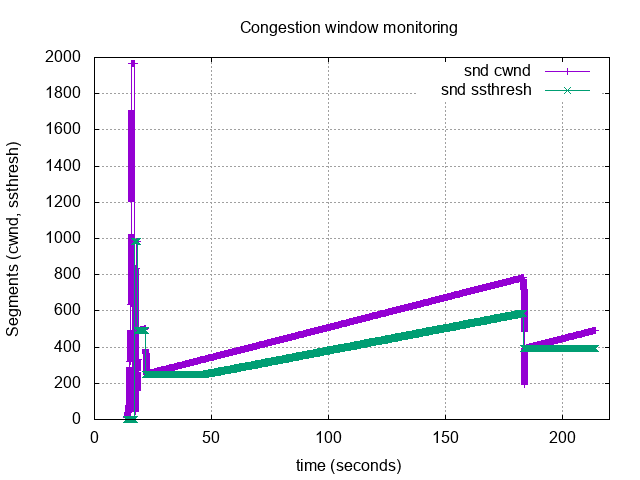
\includegraphics[scale=0.6]{images/lab1-group11-task2-question3.png}
    \caption{TCP Reno with 250ms latency and 0\% packet loss}
    \label{fig:lab1-group11-task2-question3}
\end{figure}

\subsection{Q2.4 Compare  this  graph  with  the  one  from  Q2.1,  show  the  difference  between  these  two
graphs.}

Because of the increased latency, the RTT is longer. The timeout is calculated based on the the RTT of the sent packets, they will include the larger latency and result in a larger timeout value. This is the reason why the congestion avoidance phase is running longer on the latter graph.

\newpage

\subsection{Q2.5 Plot a graph showing CWND and ssthresh versus time with
all the data you get.}

\begin{figure}[h]
    \centering
    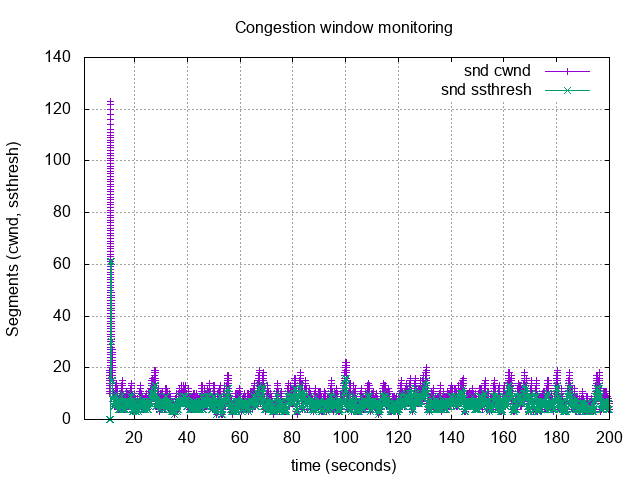
\includegraphics[scale=0.6]{images/lab1-group11-task2-question5.png}
    \caption{TCP Reno with 50ms latency and 3\% packet loss}
    \label{fig:lab1-group11-task2-question5}
\end{figure}


\subsection{Q2.6 Compare this graph with the graph of}

The major difference is that the scales significantly differ: on the earlier graph the maximum CWND is ~2300 whereas within the new capture the CWND never goes above 130. Due to the packet loss introduced, timeouts occur after a short stay in fast recover, the process enters congestion avoidance and slow start iterations. Due to the timeouts, the CWND will never have the opportunity to grow further and it will stay around the MSS 10.

\newpage

\subsection{Q2.7 Zoom in the graph of this scenario (plot some parts of
this scenario in a short duration, 10 or 20 seconds). Briefly explain
the changing process.}

\begin{figure}[h]
    \centering
    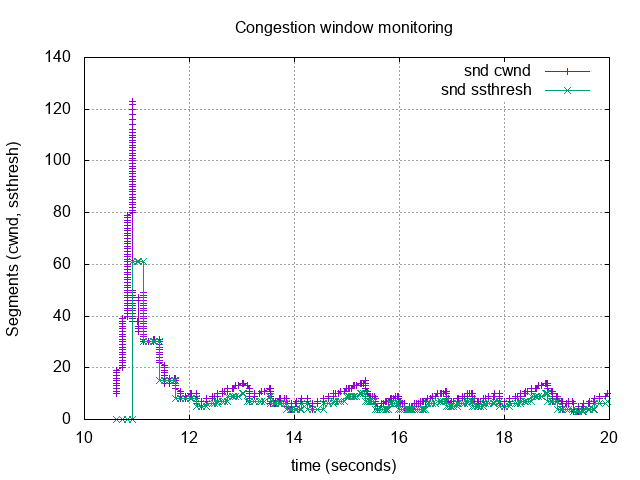
\includegraphics[scale=0.6]{images/lab1-group11-task2-question7.png}
    \caption{TCP Reno with 50ms latency and 3\% packet loss}
    \label{fig:lab1-group11-task2-question7}
\end{figure}

The same thing happens as on the previous chart, however on a lower scale. The gaps between the captured points is increased, because there are a lot of lost packets. The process is in slow start at the beginning, then it goes to iterations of fast recovery and congestion avoidance.

\subsection{Q2.8 Show a screen capture of the real throughput in this
scenario.}

\begin{figure}[h]
    \centering
    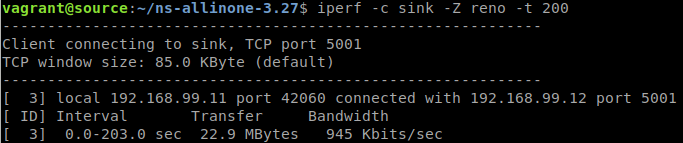
\includegraphics[scale=0.6]{images/lab1-group11-task2-question8.png}
    \caption{Real throughput of TCP Reno with 50ms latency and 3\% packet loss }
    \label{fig:lab1-group11-task2-question8}
\end{figure}

\newpage

\subsection{Q2.9 Plot a graph showing CWND and ssthresh versus time with
all the data you get.}

\begin{figure}[h]
    \centering
    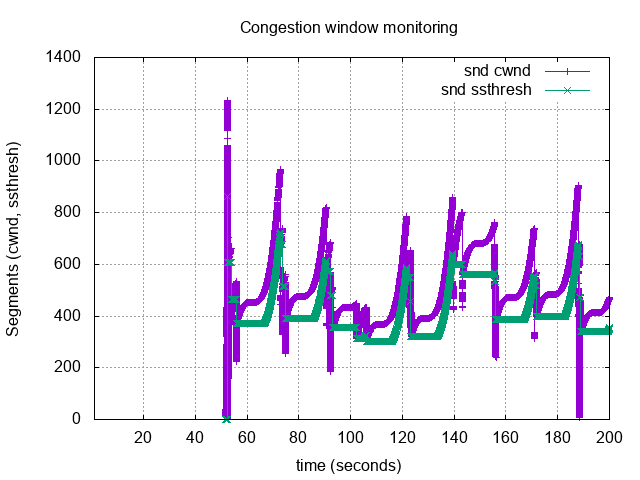
\includegraphics[scale=0.6]{images/lab1-group11-task2-question9.png}
    \caption{Cubic with 50ms latency and 0\% packet loss }
    \label{fig:lab1-group11-task2-question9}
\end{figure}

\subsection{Q2.10 Compare this graph with the graph of Q2.1 discuss and point out the major differences.}

The function that is used in CUBIC to determine the new CWND is only dependant on the packet loss, it does not include RTT. This is different from the function used in Reno, and hence the shape of the lines describing the congestion avoidance phase on the graphs look different. The same patterns are visible however: the process starts in slow start really high SSTH until it hits the first 3 dup acks, which after it enters the same iterations of fast recorver and congestion avoidance using the CUBIC mathematical formula to calculate the new CWND.

\newpage

\subsection{Q2.11 Plot a graph showing CWND and ssthresh versus time
with all the data you get.}

\begin{figure}[h]
    \centering
    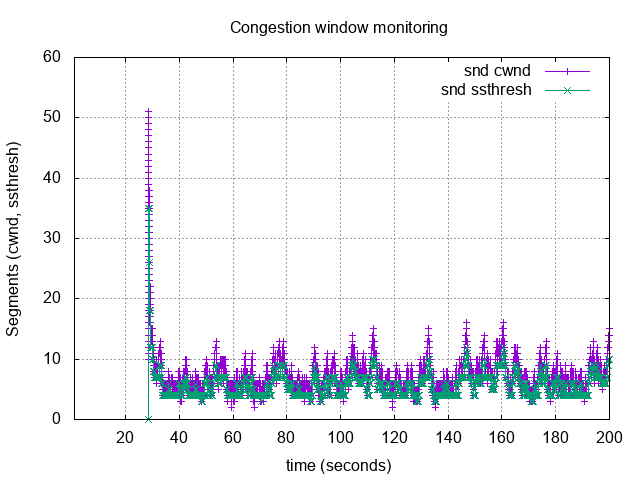
\includegraphics[scale=0.5]{images/lab1-group11-task2-question11.png}
    \caption{Cubic with 50ms latency and 3\% packet loss }
    \label{fig:lab1-group11-task2-question11}
\end{figure}


\subsection{Q2.12 Compare this graph with the graph of scenario three
and show the differences.}

Figure \ref{fig:lab1-group11-task2-question11} shows a similar behaviour that can be observed in scenario 3. The lower scale is obvious, that happens due to the increased packet losses, which introduces timeouts. The process starts between slow start and fast recovery, then enters iterations of slow start and congestion avoidance.
\newpage
\subsection{Q2.13 Zoom in the graph of this scenario (plot some parts of
this scenario in a short duration, 10 or 20 seconds). Briefly explain
the changing process and compare it with the graph of Q2.7.}

In figure \ref{fig:lab1-group11-task2-question13} the slow start phase of the process can be clearly observed at the beginning of the chart. The first thing will be noticed is the 3 dupacks, and then the first timeout occur, at which time the bounce between fast recover and slow start happened, and the process enters congestion avoidance. Due to the packet losses the process always returns to slow start and the CWND will consistently stay around the MSS 10.

\begin{figure}[h]
    \centering
    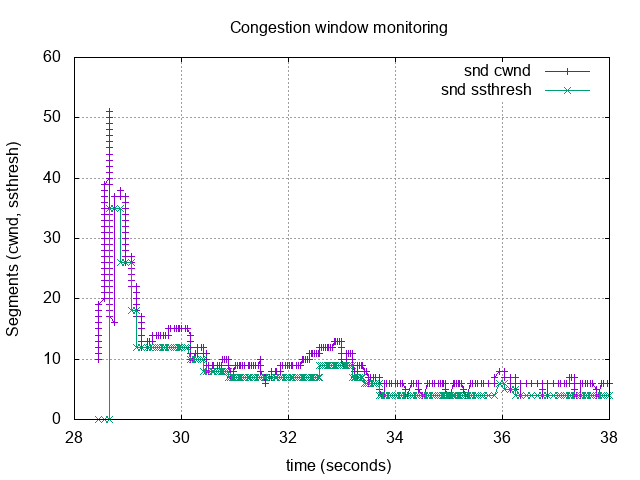
\includegraphics[scale=0.5]{images/lab1-group11-task2-question13.png}
    \caption{Cubic with 50ms latency and 3\% packet loss }
    \label{fig:lab1-group11-task2-question13}
\end{figure}

\subsection{Q2.14 Show a screen capture of the real throughput and
compare it with throughput of Q2.8.
Explain the differences.}

\begin{figure}[h]
    \centering
    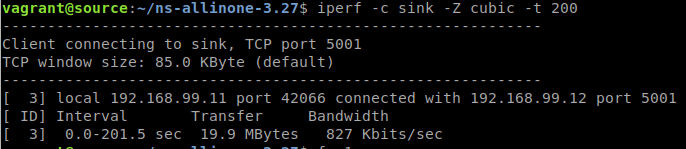
\includegraphics[scale=0.6]{images/lab1-group11-task2-question14.png}
    \caption{Real throughput of Cubic with 50ms latency and 3\% packet loss }
    \label{fig:lab1-group11-task2-question14}
\end{figure}

In figure \ref{fig:lab1-group11-task2-question14} the measured bandwidth is a little bit lower, so the resulting throughput will also be lower. This is due to the cubical function used to increase the CWND size: instead of the linear increase, the CWND is increasing slightly slower in the middle part of the cubical function - as a result, the measured bandwidth will be lower.

\subsection{Q3.1 Explain what an LFN network is. Change the simulation
parameters to your likings and demonstrate that TcpNewReno is not
suitable for LFN networks.}

To understand a Long Fat Network (LFN) network, first the Bandwidth Delay Product (BDP) should be explained. The BDP is the maximum amount of data that can be in the network at any given time, measured in bits. It is the product of the bandwidth (bits/sec) with and the RTT (sec). 
A network with a BDP larger than $10^5$ bits is called a LFN.



\subsection{Q3.2 Explain SACK does. Change the simulation parameters to
your likings and demonstrate the performance improvement with SACK.}

Selective Acknowledgements are a way to 

\subsection{Q3.3 Explain with TCP fairness is. Show the effect of
multiple flows in the simulation.}

\subsection{Q3.4 Replicate scenario 3 of the emulation: packet loss of
3\%, delay of 50 ms and transfer duration of 200sec. Use TcpNewReno.
Compare the two results.}

\subsection{Q3.5 After these experiments, please briefly describe the
difference between simulation and emulation?}

\newpage
\printbibliography

\end{document}
% Template for table used in Task 1
%
% \begin{table}
% \begin{tabular}{|c|p{25mm}|p{20mm}|c|c|}
% \hline Time (s)    & Current CWND (bytes)    & New CWND (bytes)    & New State    & Event \\
% \hline ...         &              &          &             & \\ 
% \hline ...         &              &          &             & \\ 
% \hline ...         &              &          &             & \\ 
% \hline ...         &              &          &             & \\   
% \hline  
% \end{tabular} 
% \end{table}